\documentclass[aspectratio=169]{beamer}

\useoutertheme{infolines}

\usepackage{graphicx}
\usepackage{subcaption}

\title{PNLSS Identification}
\subtitle{Post TRC Institute Meeting 5}
\author[Balaji, N. N.]{Nidish Narayanaa Balaji}
\institute[Rice U.]{Rice University, Houston, TX 77005}
\date{October 24, 2019}
\begin{document}
\maketitle{}

\begin{frame}
  \frametitle{Overview}
  \begin{columns}
    \begin{column}{0.3\linewidth}
      \vspace{-0.55cm}
      \begin{figure}[!h]
        \centering
        \begin{subfigure}{\linewidth}
          \centering
          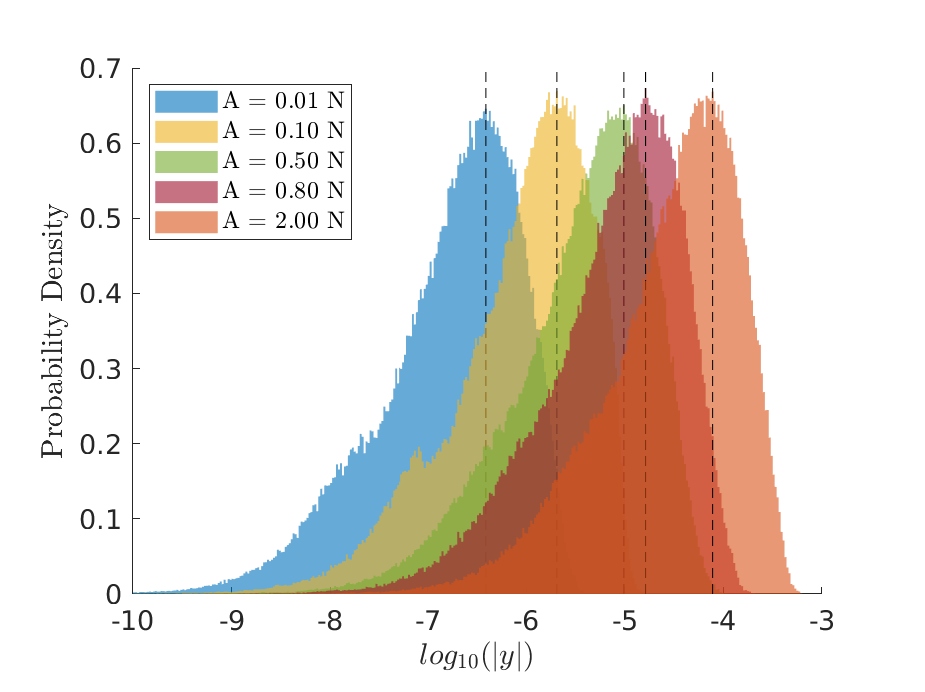
\includegraphics[width=\linewidth]{../../benchmark4/FIGURES/MSDAT_LHIST}
          \caption{Multisine Data Extent}
          \label{fig:msdat}
        \end{subfigure}
      
      \begin{subfigure}{\linewidth}
        \centering
        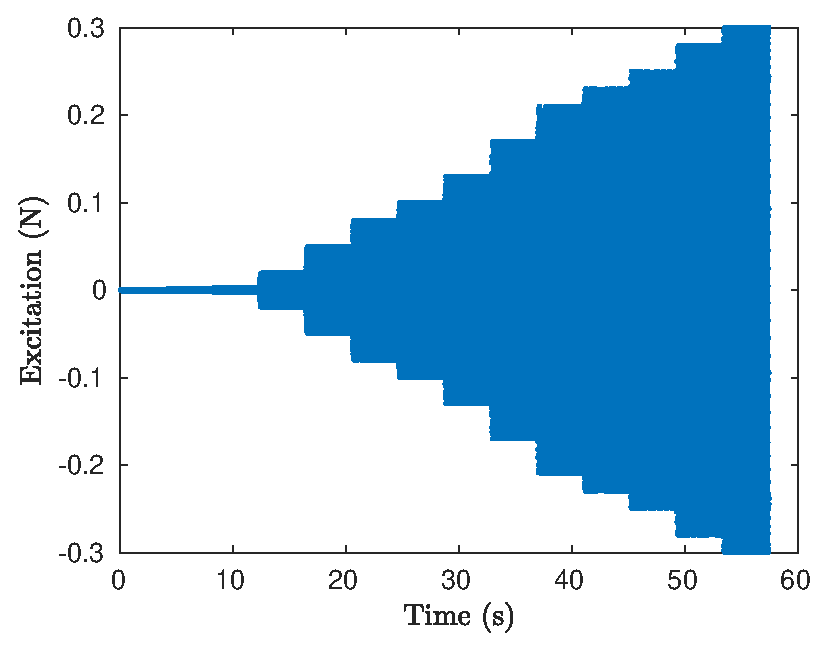
\includegraphics[width=0.7\linewidth]{../../benchmark4/FIGURES/PLL_EXCITATION}
        \caption{PLL Excitation}
        \label{fig:pllu}
      \end{subfigure}
    \end{figure}
    \end{column}
    \begin{column}{0.7\linewidth}
      \vspace{-1cm}
      \begin{itemize}
      \item Current set of slides contain results for
        \textbf{benchmark 4}, the beam with elastic dry-friction
        element
      \item The left shows a histogram of the magnitude of the
        multi-sine response data
      \item PNLSS models using this data is used to train the initial
        guesses for the identification on the PLL data
      \item PNLSS optimization is conducted using the \textbf{FULL
          DATA} from the simulated experiments, i.e., \textbf{this
          includes the transients} inherent
      \item This procedure was adopted since it maximized the amount
        of data we used for PNLSS
      \end{itemize}
    \end{column}
  \end{columns}
\end{frame}

\begin{frame}[allowframebreaks]
  \frametitle{Multi-sine PNLSS models: Performance on PLL data}
  \vspace{-0.5cm}
  \begin{figure}[!h]
    \centering
    \begin{subfigure}[!h]{0.2\linewidth}
      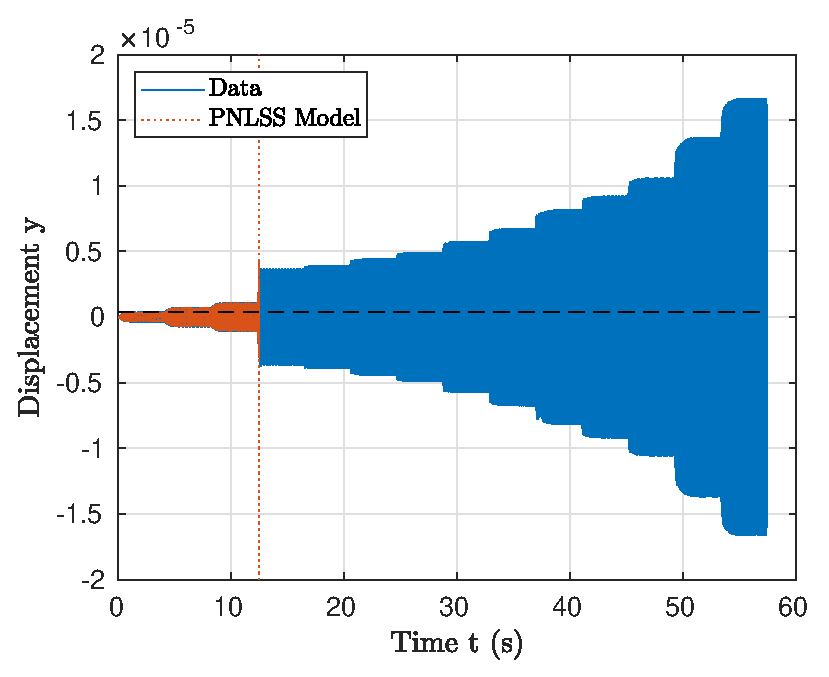
\includegraphics[width=\linewidth]{../../benchmark4/FIGURES/PNLSS_PLL_TRESP_famp001_nx23}
      \caption{A = 0.01 N}      
    \end{subfigure}%
    \begin{subfigure}[!h]{0.2\linewidth}
      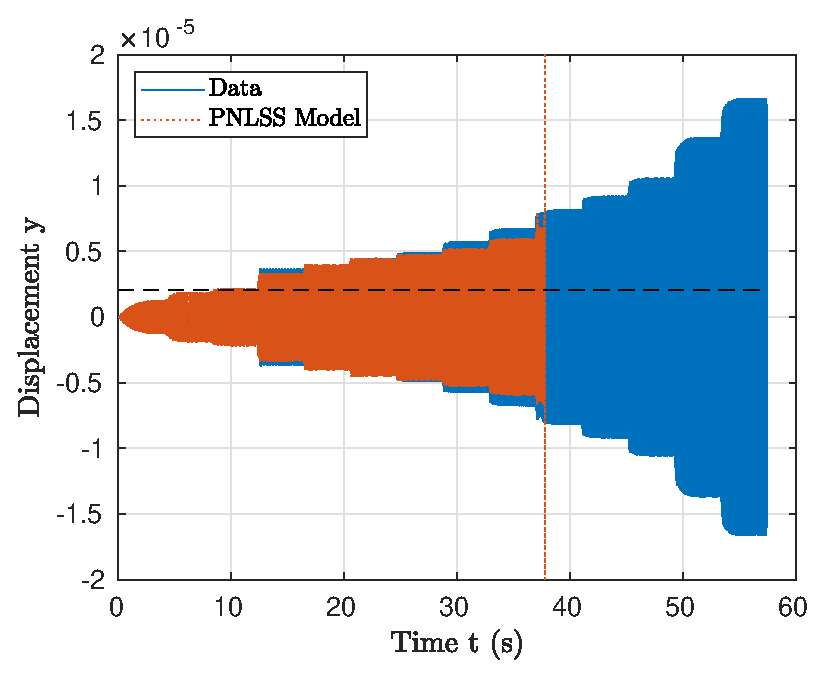
\includegraphics[width=\linewidth]{../../benchmark4/FIGURES/PNLSS_PLL_TRESP_famp01_nx23}
      \caption{A = 0.10 N}      
    \end{subfigure}%
    \begin{subfigure}[!h]{0.2\linewidth}
      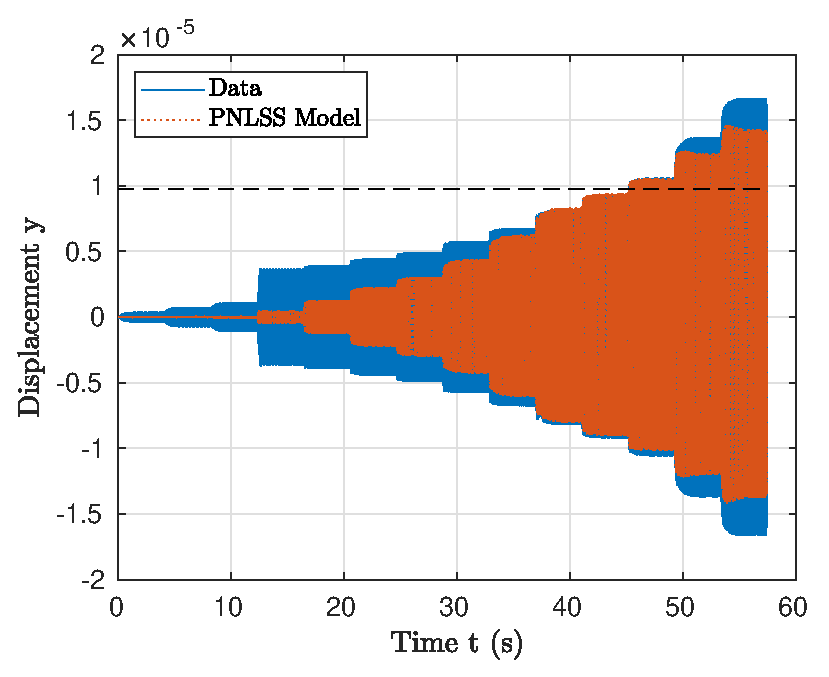
\includegraphics[width=\linewidth]{../../benchmark4/FIGURES/PNLSS_PLL_TRESP_famp05_nx23}
      \caption{A = 0.50 N}      
    \end{subfigure}%
    \begin{subfigure}[!h]{0.2\linewidth}
      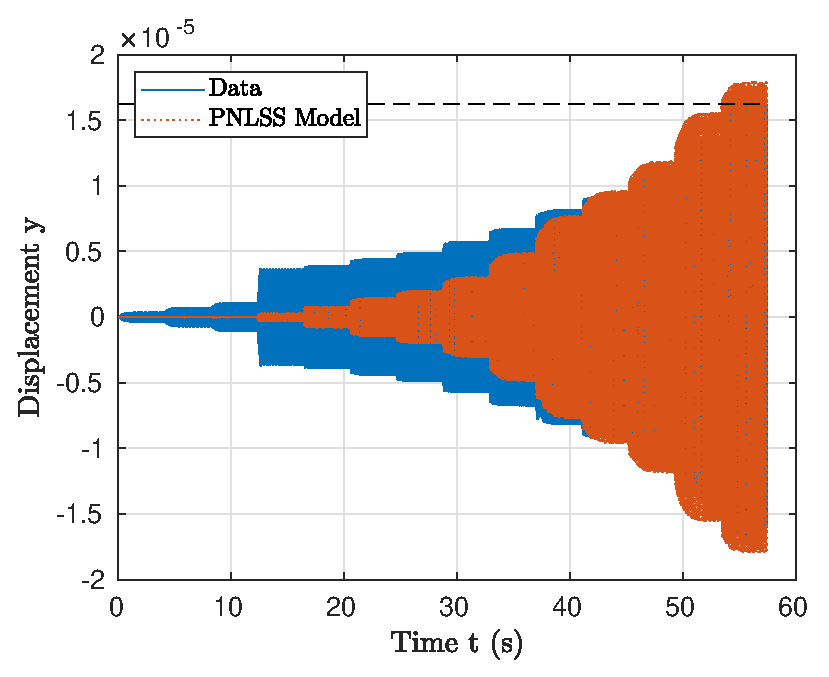
\includegraphics[width=\linewidth]{../../benchmark4/FIGURES/PNLSS_PLL_TRESP_famp08_nx23}
      \caption{A = 0.80 N}      
    \end{subfigure}%
    \begin{subfigure}[!h]{0.2\linewidth}
      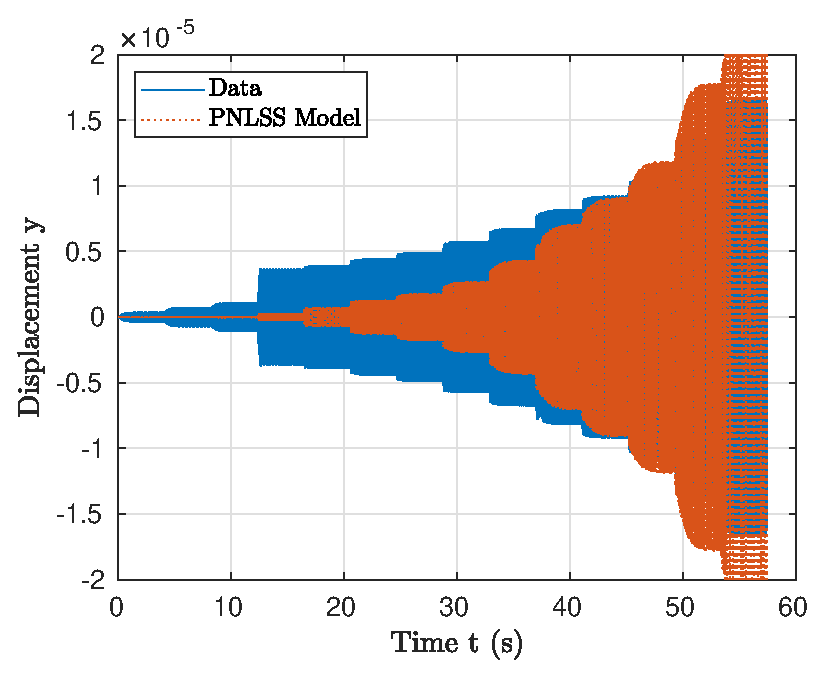
\includegraphics[width=\linewidth]{../../benchmark4/FIGURES/PNLSS_PLL_TRESP_famp20_nx23}
      \caption{A = 2.00 N}
    \end{subfigure}
    \caption{Time domain performance on PLL excitation}
    \label{fig:sd}
  \end{figure}
  \vspace{-1cm}
  \begin{itemize}
  \item Note that identification was carried out on \textbf{multisine
      data}. We're now just looking at how those models perform on the
    pll data
  \item Black dashed line indicates ``mode'' of the multi-sine
    response amplitude used for training the PNLSS models in each case 
  \item Note that the models identified with the lower levels (A =
    0.01 N, 0.1 N) seem to be unstable beyond a certain point
  \end{itemize}
  \begin{figure}[!h]
    \centering
    \begin{subfigure}[!h]{0.2\linewidth}
      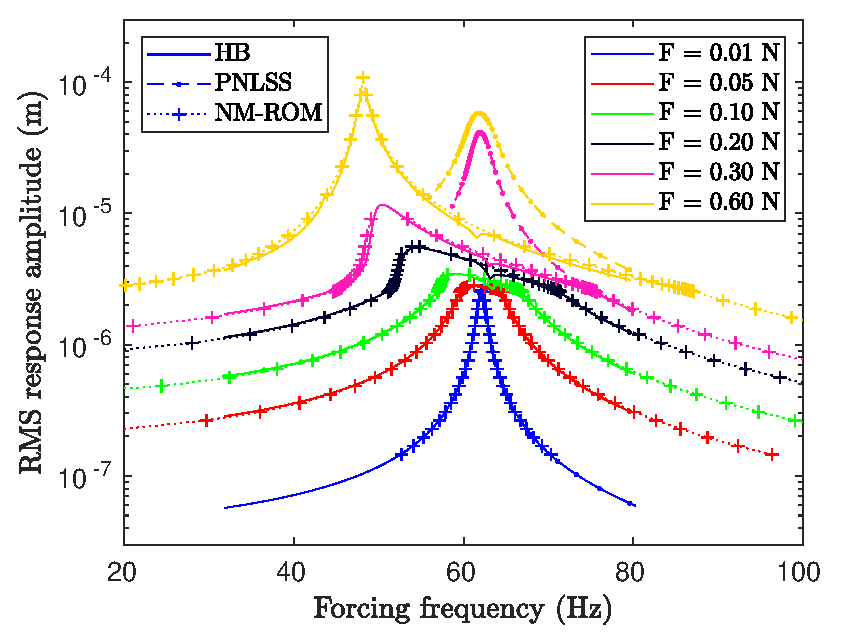
\includegraphics[width=\linewidth]{../../benchmark4/extabs_fig/b4_fresp_comp_famp001_nx23}
      \caption{A = 0.01 N}
    \end{subfigure}%
    \begin{subfigure}[!h]{0.2\linewidth}
      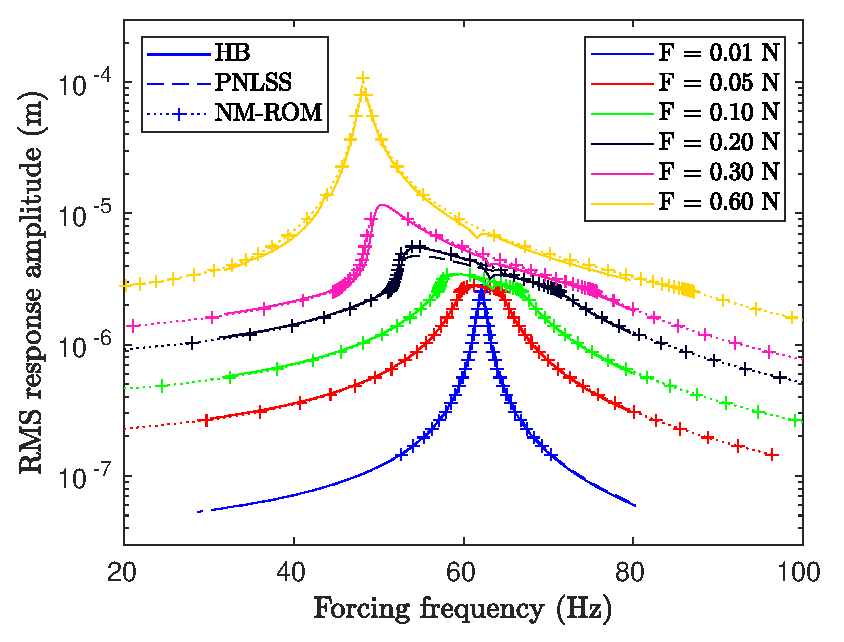
\includegraphics[width=\linewidth]{../../benchmark4/extabs_fig/b4_fresp_comp_famp01_nx23}
      \caption{A = 0.10 N}
    \end{subfigure}%
    \begin{subfigure}[!h]{0.2\linewidth}
      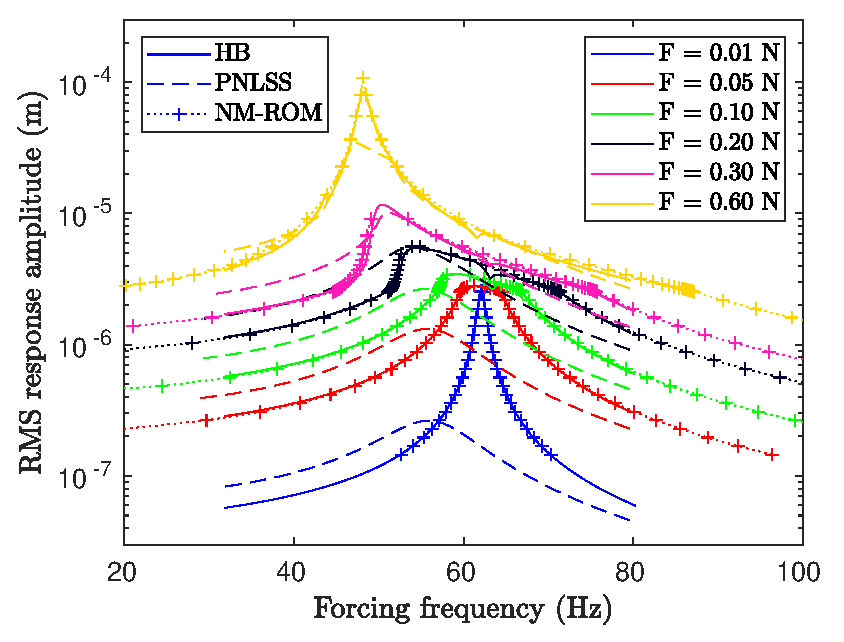
\includegraphics[width=\linewidth]{../../benchmark4/extabs_fig/b4_fresp_comp_famp05_nx23}
      \caption{A = 0.50 N}
    \end{subfigure}%
    \begin{subfigure}[!h]{0.2\linewidth}
      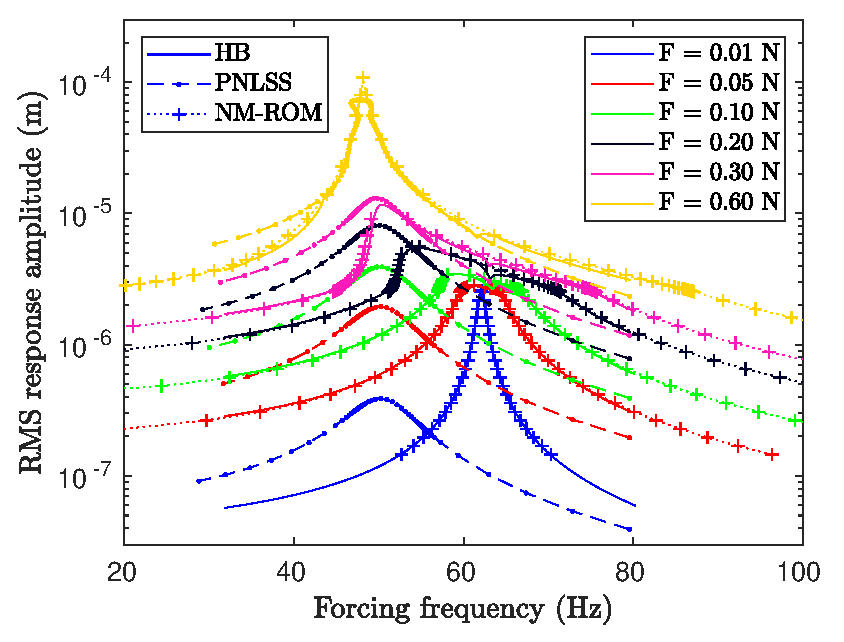
\includegraphics[width=\linewidth]{../../benchmark4/extabs_fig/b4_fresp_comp_famp08_nx23}
      \caption{A = 0.80 N}
    \end{subfigure}%
    \begin{subfigure}[!h]{0.2\linewidth}
      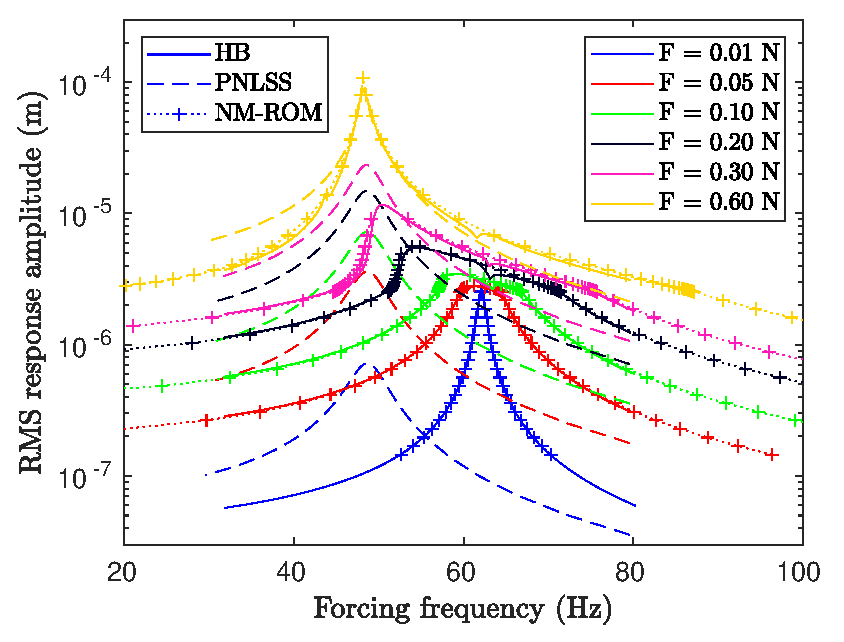
\includegraphics[width=\linewidth]{../../benchmark4/extabs_fig/b4_fresp_comp_famp20_nx23}
      \caption{A = 2.00 N}
    \end{subfigure}%
    \caption{Corresponding frequency responses of the PNLSS models
      employed before}
  \end{figure}
  \begin{itemize}
  \item The procedure used for training these PNLSS modes was:
    \begin{itemize}
    \item BLA from A = 0.01 N data set as initial guess model for
      PNLSS on A = 0.01 N data set
    \item PNLSS on A = 0.01 N set as initial guess model for PNLSS on
      A = 0.10 N data set, etc.\\
      \hspace{2cm}\vdots
    \end{itemize}
  \end{itemize}
\end{frame}

\begin{frame}[allowframebreaks]
  \frametitle{PNLSS Trained on PLL data with different multisine PNLSS
  models as initial guesses}
  \begin{figure}[!h]
    \centering
    \begin{subfigure}[!h]{0.2\linewidth}
      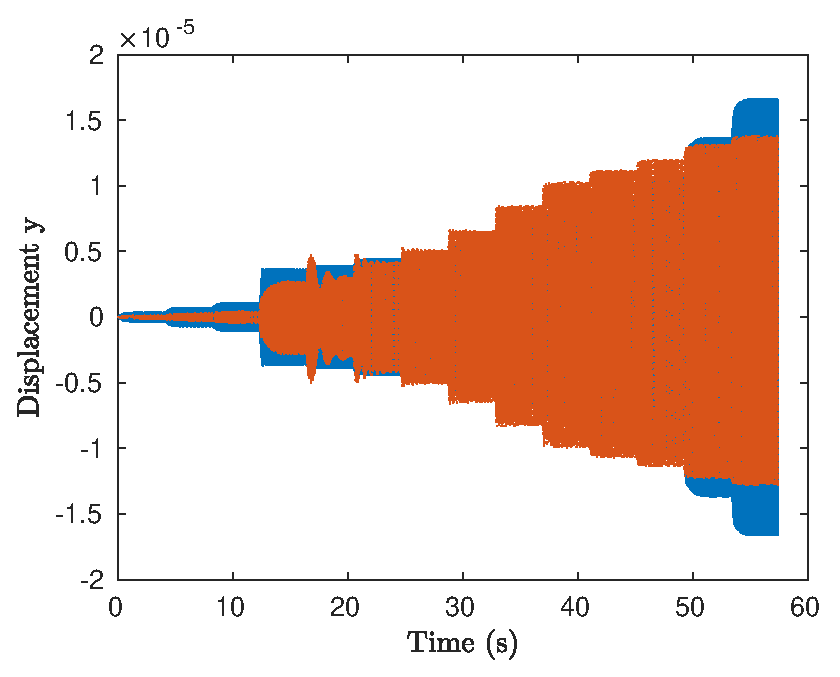
\includegraphics[width=\linewidth]{../../benchmark4/FIGURES/TDOMPERF_PNLSS_PLL_famp001_nx23}
      \caption{A = 0.01 N}
    \end{subfigure}%
    \begin{subfigure}[!h]{0.2\linewidth}
      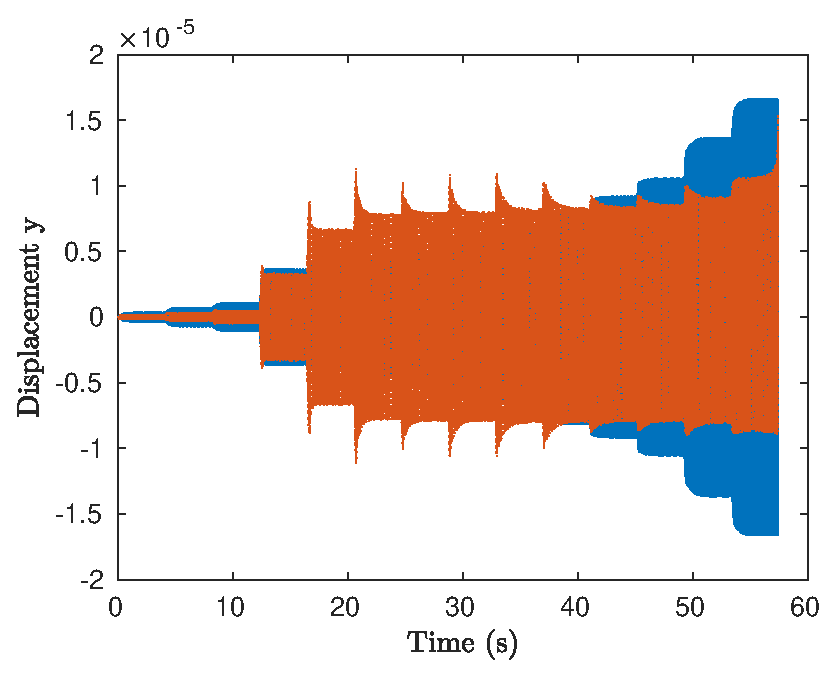
\includegraphics[width=\linewidth]{../../benchmark4/FIGURES/TDOMPERF_PNLSS_PLL_famp01_nx23} 
      \caption{A = 0.10 N}     
    \end{subfigure}%
    \begin{subfigure}[!h]{0.2\linewidth}
      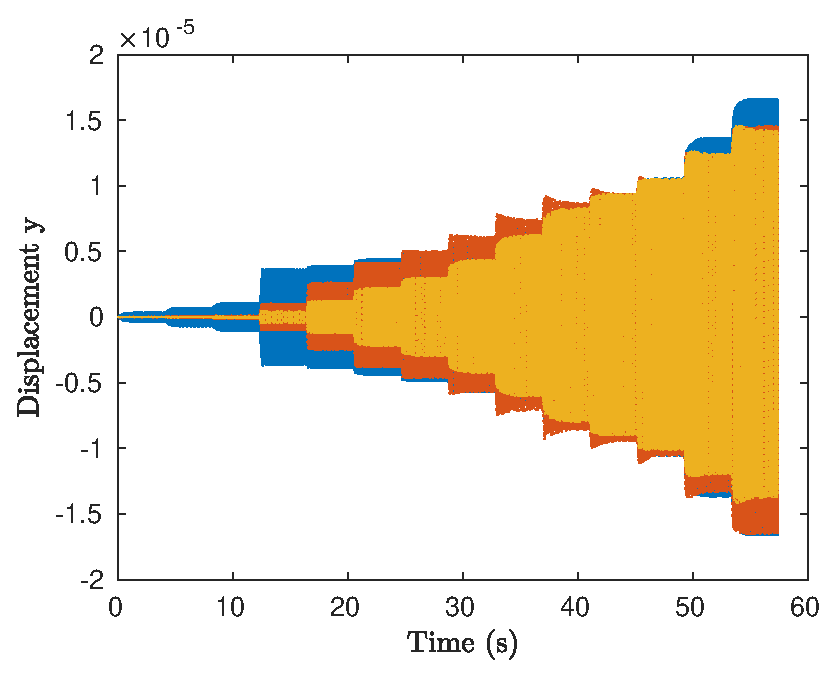
\includegraphics[width=\linewidth]{../../benchmark4/FIGURES/TDOMPERF_PNLSS_PLL_famp05_nx23}
      \caption{A = 0.50 N}      
    \end{subfigure}%
    \begin{subfigure}[!h]{0.2\linewidth}
      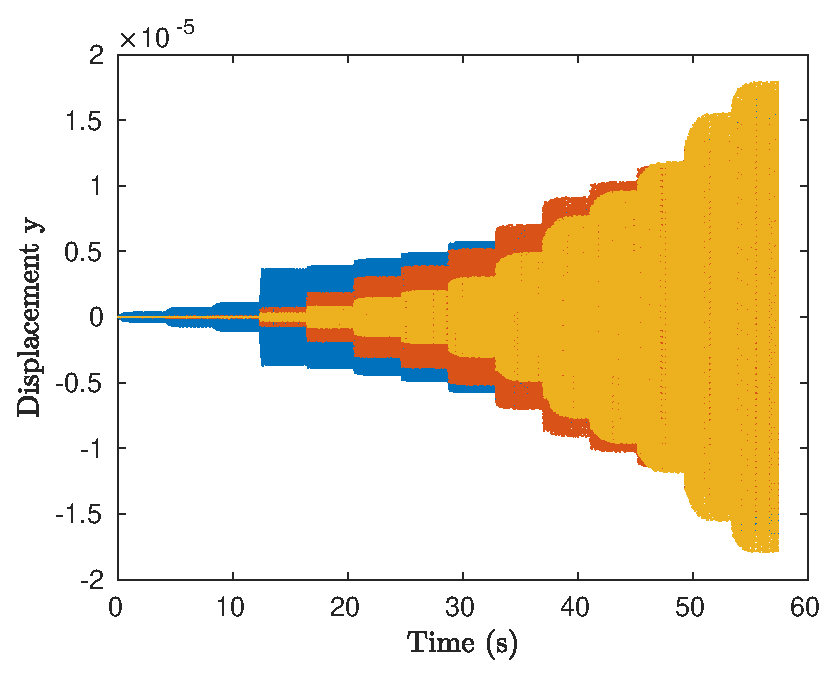
\includegraphics[width=\linewidth]{../../benchmark4/FIGURES/TDOMPERF_PNLSS_PLL_famp08_nx23}
      \caption{A = 0.80 N}      
    \end{subfigure}%
    \begin{subfigure}[!h]{0.2\linewidth}
      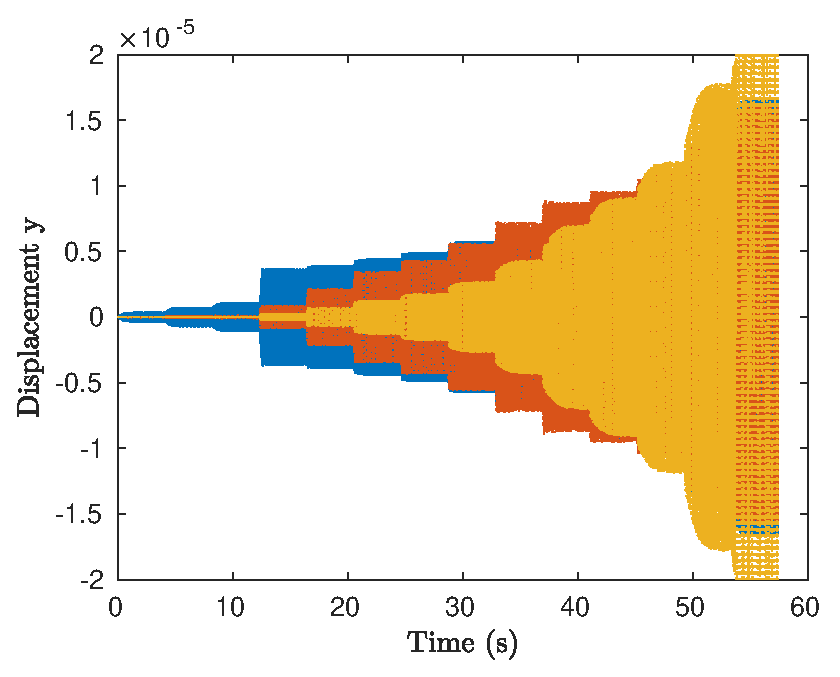
\includegraphics[width=\linewidth]{../../benchmark4/FIGURES/TDOMPERF_PNLSS_PLL_famp20_nx23}
      \caption{A = 2.00 N}      
    \end{subfigure}
    \caption{PNLSS optimization on PLL data}
  \end{figure}
  \vspace{-1cm}
  \begin{itemize}
  \item We're now looking at the performance of PNLSS models
    trained with PLL data. 
  \item \textbf{Top}: Yellow is initialized model; orange is
    PNLSS-optimized model
  \item Note that the jacobian apparently has NAN's for PNLSS models
    trained with very low amplitude data (A = 0.01 N, 0.10 N). I had
    to re-initialize the non-linear coefficients in this case
  \end{itemize}

  \begin{figure}[!h]
    \centering
    \begin{subfigure}[!h]{0.2\linewidth}
      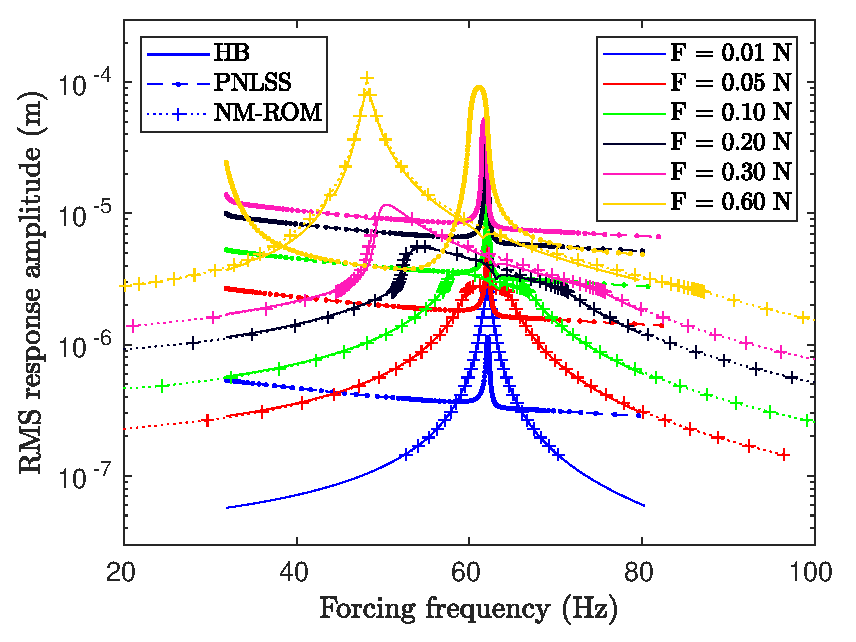
\includegraphics[width=\linewidth]{../../benchmark4/extabs_fig/b4_fresp_comp_pll_famp001_nx23}
      \caption{A = 0.01 N}
    \end{subfigure}%
    \begin{subfigure}[!h]{0.2\linewidth}
      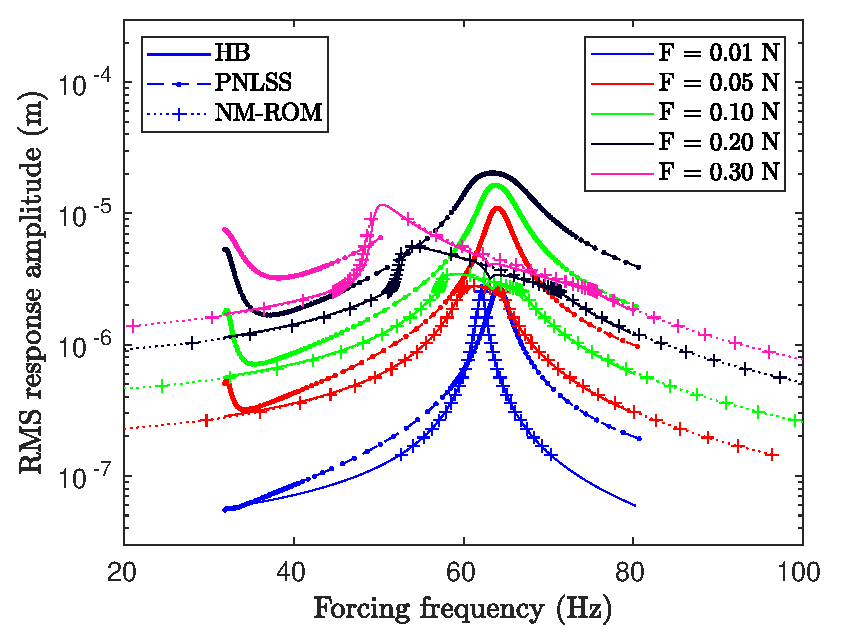
\includegraphics[width=\linewidth]{../../benchmark4/extabs_fig/b4_fresp_comp_pll_famp01_nx23}
      \caption{A = 0.10 N}
    \end{subfigure}%
    \begin{subfigure}[!h]{0.2\linewidth}
      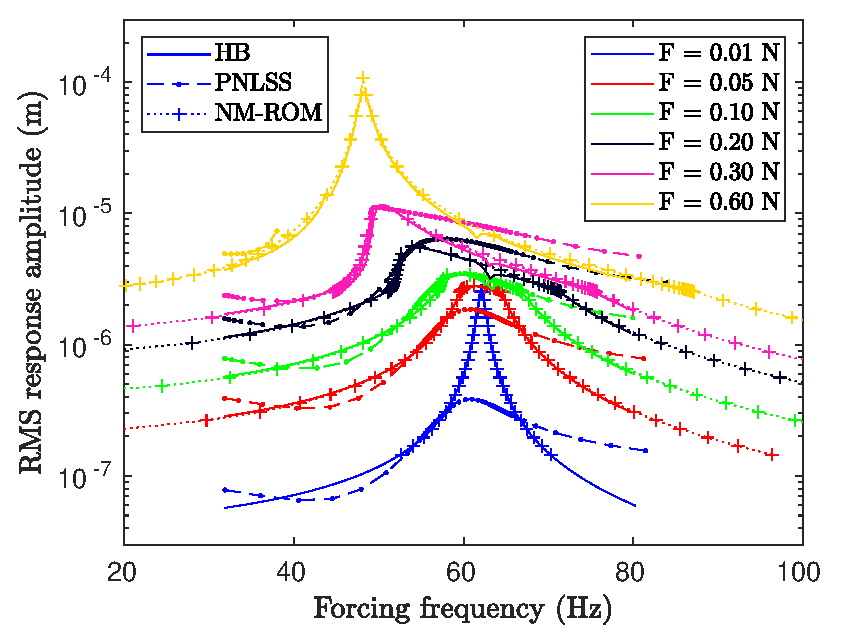
\includegraphics[width=\linewidth]{../../benchmark4/extabs_fig/b4_fresp_comp_pll_famp05_nx23}
      \caption{A = 0.50 N}
    \end{subfigure}%
    \begin{subfigure}[!h]{0.2\linewidth}
      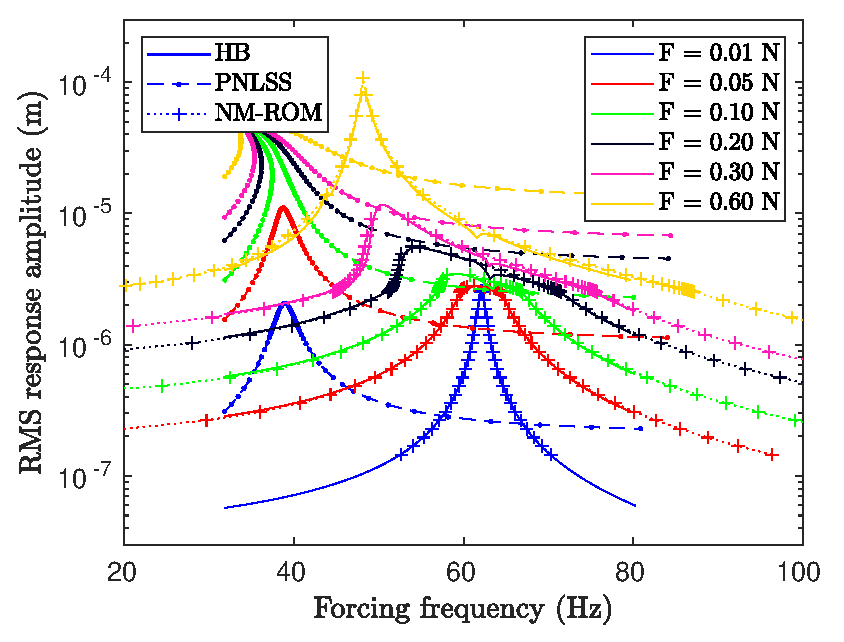
\includegraphics[width=\linewidth]{../../benchmark4/extabs_fig/b4_fresp_comp_pll_famp08_nx23}
      \caption{A = 0.80 N}
    \end{subfigure}%
    \begin{subfigure}[!h]{0.2\linewidth}
      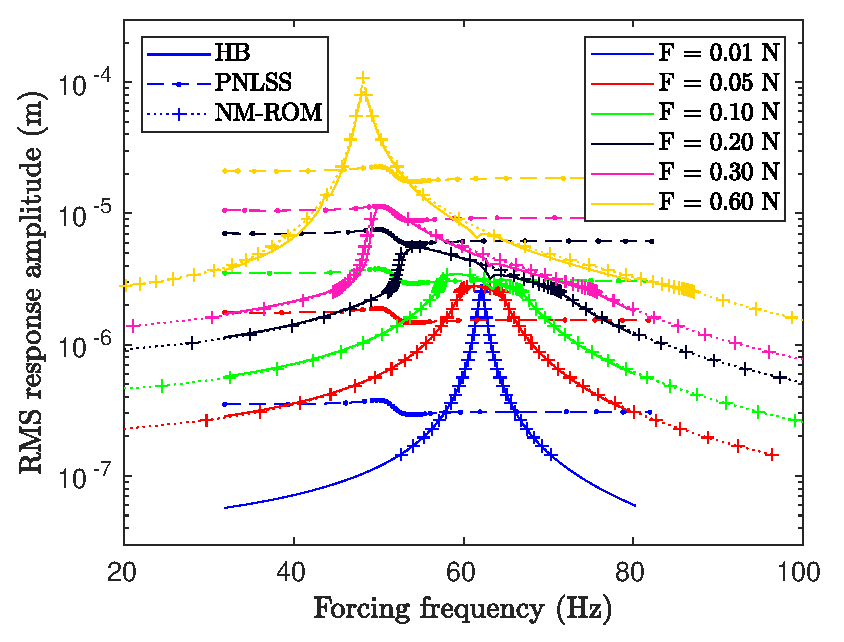
\includegraphics[width=\linewidth]{../../benchmark4/extabs_fig/b4_fresp_comp_pll_famp20_nx23}
      \caption{A = 2.00 N}
    \end{subfigure}%
    \caption{Frequency responses of PNLSS models optimized on PLL
      data. Different subfigures indicate different initializations.}
  \end{figure}
  \vspace{-0.8cm}
  \begin{itemize}
  \item Although, the model initialized at A = 0.50 N seems to capture
    the stiffness non-linearity, it does not represent the amplitudes
    very well.
  \item \textit{I am not sure if this is indication that the elastic-dry
    friction non-linearity may not be captured using the polynomial
    bases in PNLSS.}
  \end{itemize}
\end{frame}

\begin{frame}
  \frametitle{Shift in Natural Frequency of Underlying Linear Systems}
  \framesubtitle{Comparison between linear part of PNLSS model
    identified from Multi-sine data and PLL data} 

  \begin{table}[!h]
    \centering
    \begin{tabular}{ccc}
      \hline\hline
      Multisine & PNLSS from & PNLSS from PLL data\\
      Amplitude (N) & Multisine data (MSPNLSS) & initialized with MSPNLSS \\
      \hline
      0.01 & 62.0921 Hz & 62.1493 Hz \\
      0.10 & 62.2387 Hz & 62.1510 Hz \\
      0.50 & 56.2641 Hz & 59.9767 Hz \\
      0.80 & 50.3833 Hz & 38.8631 Hz \\
      2.00 & 48.7089 Hz & 51.4134 Hz \\\hline\hline
    \end{tabular}
    \caption{Eigenfrequencies from the linear part of the PNLSS models
    identified from the multisine data and the PLL data respectively.}
    \label{tab:table}
  \end{table}
\end{frame}

\end{document}
%%% Local Variables:
%%% mode: latex
%%% TeX-master: t
%%% End:
